% !TeX root = ..\main.tex
\npchapter{Grundlagen} \label{Grundlagen}
Dieses Kapitel stellt die benötigten Grundlagen vor, die für das Verständnis der darauffolgenden Kapitel notwendig sind. Hierzu zählen die Vorstellung von Node.js und Bun sowie weiterer Grundlagen zu Performanceanalysen.

\section{Node.js} \label{sec:Node.js}
Node.js ist ein beliebtes Tool für eine große Varianz an Projekten, darunter leichtgewichtige Webservices, dynamische Webanwendungen und Tools für die Kommandozeile. Es handelt sich um eine Open Source, platformunabhängige Laufzeitumgebung, die es ermöglicht JavaScript außerhalb des Browsers auszuführen. Node.js verwendet die V8 JavaScript Engine von Google, die auch in Google Chrome kommt. Dies ermöglicht Node.js eine hohe Performance, weshalb Unternehmen wie Netflix und Uber Node.js in ihren Softwareprojekten einsetzen. \cite{OpenJSFoundation.2022} \\

\begin{figure}[h]
	\centering
	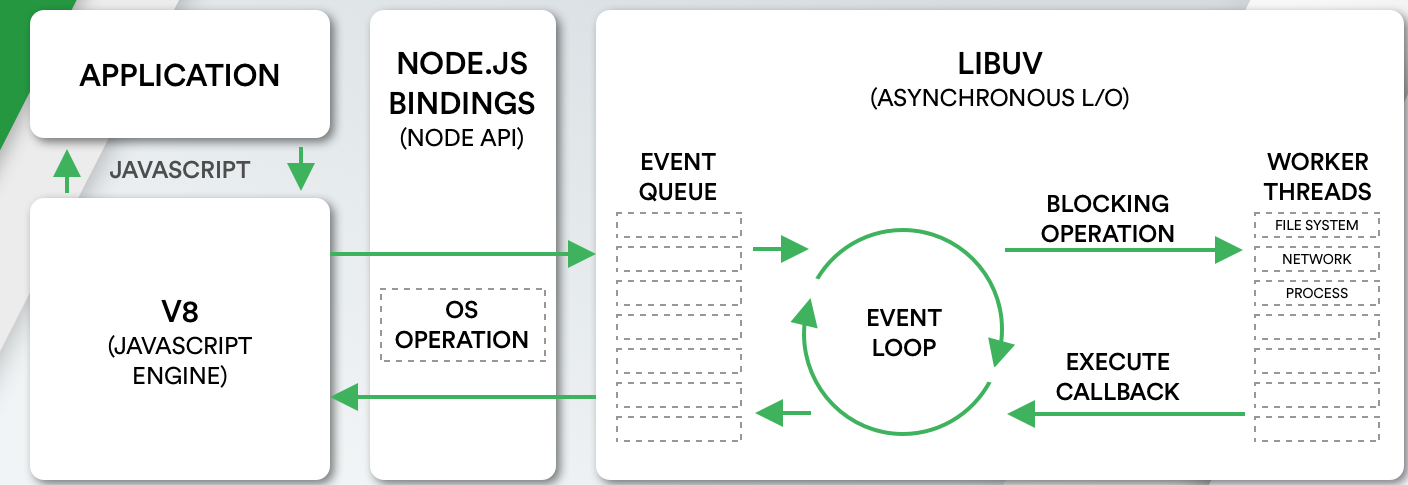
\includegraphics[width=\linewidth]{./images/NodeJsArchitecture}
	\caption{Node.js Architektur}
	\label{fig:nodejs-architecture}
\end{figure}
 
\noindent
Abbildung \ref{fig:nodejs-architecture} zeigt die Architektur von Node.js. Grundsätzlich nutzt Node.js nur einen Thread und erstellt nicht für jede neue Anfrage einen neuen Thread. Sobald eine Applikation gestartet wird, wird in dem einzigen Thread der Node.js-Prozess gestartet. Die V8 Engine optimiert den Maschinencode zusätzlich an häufig benötigten Stellen, wobei dies nicht sofort geschieht, da die Übersetzung in Maschinencode aufgrund der Just-in-Time-Kompilierung zeitsensitive Aufgabe darstellt. Darüber hinaus ist in der Engine ein Garbage Collector integriert, der nicht mehr verwendete Objekte löscht.  \cite{Springer.2022} \newline 
Für weitere Aufgaben setzt Node.js auf Bibliotheken, die fertige und etablierte Lösungsansätze für häufig benötigte Aufgaben zur Verfügung stellen. Nur für Aufgaben, für die es keine etablierte Bibliothek gibt, werden eigene Implementierungen verwendet. Im Folgenden werden die wichtigsten Komponenten vorgestellt. \cite{Springer.2022} \\

\noindent
\textbf{Event Loop} \newline
Node.js verwendet eine eventgesteuerte Architektur. Anstatt den Quellcode linear auszuführen, werden definierte Events ausgelöst, für die zuvor Callback-Funktionen registriert wurden. Dieses Konzept wird genutzt, um eine hohe Anzahl von asynchronen Aufgaben zu bewältigen. Um dabei den einzelnen Thread der Anwendung nicht zu blockieren, werden Lese- und Schreiboperationen an den Event Loop ausgelagert.  Wenn auf externe Ressourcen zugegriffen werden muss, leitet der Event Loop die Anfrage weiter, und die registrierte Callback-Funktion gibt die Anfrage an das Betriebssystem weiter. In der Zwischenzeit kann Node.js andere Operationen ausführen. Das Ergebnis der externen Operation wird dann über den Event Loop zurückgeliefert. \cite{Springer.2022} \newline 
Während der Laufzeit werden viele Events erzeugt und in einer Message Queue, der Event Queue, nacheinander gespeichert. Node.js nutzt FIFO und beginnt demnach mit der Verarbeitung der ältesten Events und arbeitet sich durch die Queue, bis keine Events mehr vorhanden sind. \cite{OpenJSFoundation.o.J.} \\

\noindent
\textbf{Libuv} \newline
Der Event Loop von Node.js basiert ursprünglich auf der Bibliothek libev. Diese ist in C geschrieben und für ihre hohe Leistung und umfangreichen Features bekannt. Allerdings stützt sich libev auf native UNIX-Funktionen, die unter Windows auf andere Weise verfügbar sind. Daher dient Libuv als Abstraktionsebene zwischen Node.js und den darunter liegenden Bibliotheken für den Event Loop, um die Laufzeitumgebung auf allen Plattformen nutzen zu können. Libuv verwaltet alle asynchronen I/O-Operationen, einschließlich Dateisystemzugriffe und asynchrone TCP- und UDP-Verbindungen. \cite{Springer.2022} \\

\noindent
Darüber hinaus bringt Node.js den Node Package Manager (NPM) mit sich. Dieser Paketmanager ist entscheidend für den Erfolg von Node.js, da es im September 2022 mehr als 2,1 Millionen Pakete in diesem Ökosystem gibt. Es gibt somit ein Paket für nahezu alle Anwendungsfälle. Ursprünglich wurde NPM entwickelt, um Abhängigkeiten in Projekten zu verwalten, wird aber mittlerweile auch als Werkzeug für JavaScript im Frontend unterstützt. \cite{OpenJSFoundation.2022}\\

\noindent
Zusammenfassend zeichnet sich Node.js durch eine eventgesteuerte Architektur und durch ein nicht blockierendes Modell für Ein- und Ausgabeoperationen aus, was es leichtgewichtig und effizient macht. Dies hat verschiedene Vor- und Nachteile. \newline
Zu den Vorteilen gehören eine hohe Performance durch die Nutzung der V8 JavaScript Engine und die Plattformunabhängigkeit. Eine weitere Stärke ist die große und aktive Community an Entwicklern. Dank der Popularität gibt es viele etablierte Lösungsansätze, die den Entwicklungsprozess beschleunigen und vereinfachen. \cite{OpenJSFoundation.2022} Node.js ermöglicht die Verwendung der JavaScript-Sprache sowohl auf der Server- als auch auf der Clientseite. Dies vereinfacht die Entwicklung von Full-Stack-Anwendungen und erleichtert Entwicklern den Einstieg. \cite{Brown.November2019} Das effiziente nicht blockierende I/O-Modell von Node.js ermöglicht es, mehrere gleichzeitige Anfragen effizient zu verarbeiten und eignet sich daher gut für anwendungsspezifische Aufgaben, die viele gleichzeitige Verbindungen erfordern. \todo{Quelle einfügen} \todo{Skalierbarkeit?} \newline
Allerdings existieren auch Nachteile bei der Verwendung von Node.js. Das Single-Threaded-Modell kann bei rechenintensiven oder CPU-lastigen Aufgaben zu Engpässen führen, da es nur einen Hauptthread für die Ausführung von Code gibt. Bei komplexen Anwendungen kann die Verwaltung von Callbacks und Promises zur Bewältigung von asynchronem Code kompliziert werden. \todo{Quelle einfügen} \newline
Ein weiterer Nachteil ist, dass Node.js im Vergleich zu einigen anderen Laufzeitumgebungen über eine begrenzte Standardbibliothek verfügt, sodass Entwickler häufig auf externe Module und Pakete zurückgreifen müssen. Darüber hinaus kann die Qualität einiger NPM-Pakete variieren, und schlecht gewartete Module können zu Kompatibilitätsproblemen und Sicherheitsrisiken führen. \todo{Quelle einfügen} \newline
Insgesamt ist Node.js eine leistungsfähige und vielseitige Laufzeitumgebung, die sich gut für bestimmte Anwendungsfälle eignet, insbesondere wenn es darum geht, skalierbare und asynchrone Anwendungen zu entwickeln. Dennoch sollten Entwickler die Vor- und Nachteile sorgfältig abwägen und die Anforderungen ihres Projekts berücksichtigen, um zu entscheiden, ob Node.js die richtige Wahl ist. \todo{Quelle einfügen}



\section{Bun} \label{sec:Node}
TODO\\

\section{Performanceanalyse} \label{sec:Performanceanalyse}
TODO\\
